\documentclass[a4paper]{article}
\usepackage[a4paper, top = 0.5cm, bottom = 0.5cm, left = 1.5cm, right = 1.5cm]{geometry}
\usepackage{graphicx} % Required for inserting images
\usepackage{listings}
\usepackage{amsmath}
\usepackage{hyperref}

\title{EE 236 Devices Lab \\ Lab - 05}
\author{Anupam Rawat, 22b3982}
\date{${08^{th}}$ September, 2024}

\begin{document}
\hypertarget{page1} 
\maketitle
\begin{center}
    \section*{Temperature Dependence of Solar Cell I/V Characteristics}    
\end{center}


\section{Dark forward characteristics at different temperatures}

\subsection{Aim of the experiment}
Observe the I-V Characteristics of the Solar Cell in forward bias and in dark conditions.

\subsection{Design}
\begin{figure}[h!]
    \centering
    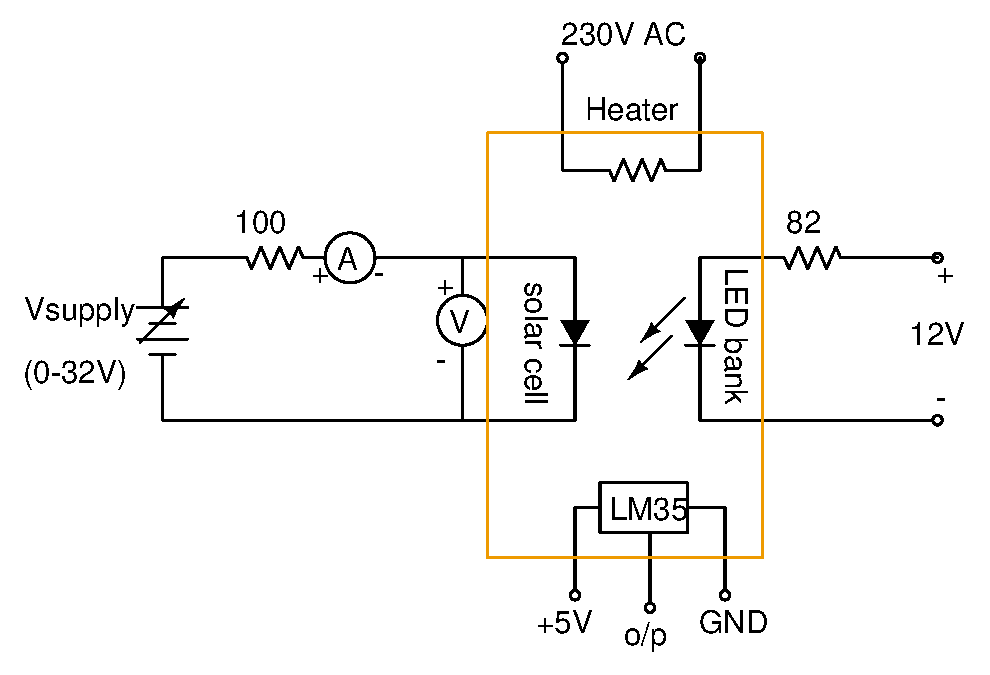
\includegraphics[width=0.75\linewidth]{Ckt_Design_Experiment_1.eps}
    \caption{Caption}
    \label{fig:enter-label}
\end{figure}

\subsection{Simulation}
\subsubsection{Code}
\begin{lstlisting}
IV characteristics of Solar Cell
Solar Cell description was given in a file format
.include "../solar_cell.txt"
Vin 1 0 dc 0
X1 1 2 solar_cell
r1 2 0 100

.dc Vin -2 2 0.01
.temp 35
.control
run
plot -i(vin) vs {v(1)-v(2)}
wrdata dark_35C.txt -i(vin) {v(1)-v(2)} 
.endc
.end
\end{lstlisting}
\newpage
\hypertarget{page2}{}

\subsubsection{Results}
\begin{figure}[h!]
    \centering
    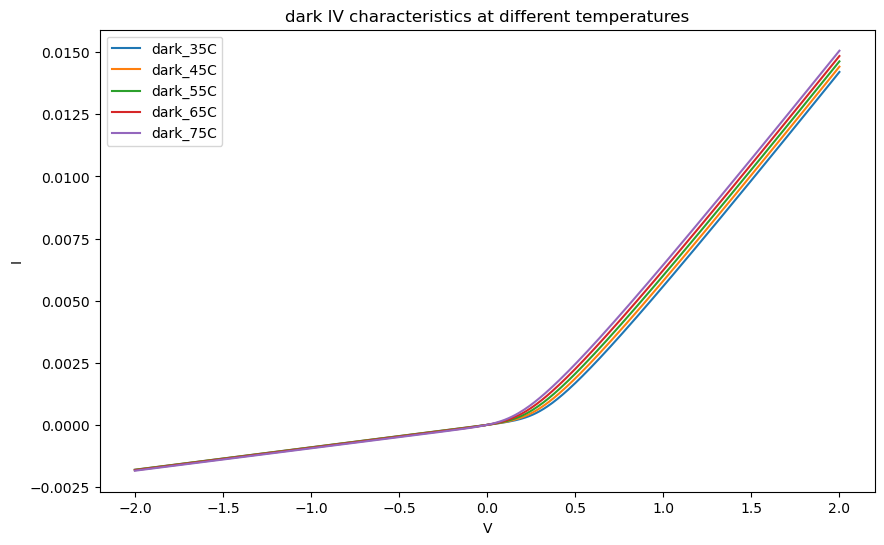
\includegraphics[width=0.9\linewidth]{Lab_5/Pre_Lab/Dark_IV.png}
    \caption{Dark I/V Characteristic across various temperatures - Simulation}
\end{figure}

\begin{figure}[h!]
    \centering
    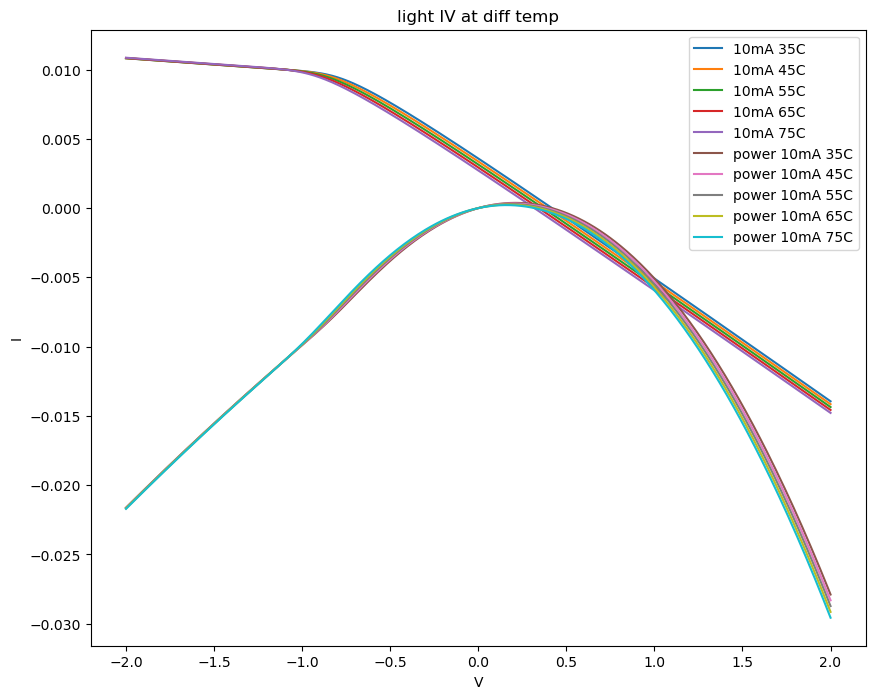
\includegraphics[width=0.9\linewidth]{Lab_5/Pre_Lab/Illuminated_IV.png}
    \caption{Illuminated I/V Characteristic across various temperatures - Simulation}
\end{figure}

\newpage
\hypertarget{page3}{}

\subsubsection{Simulation Results}
The values of fill factors are obtained using this equation:
\[
\text{Fill Factor} = \frac{V_{MP} \times I_{MP}}{V_{OC} \times I_{SC}}
\]
\begin{table}[h!]
    \centering
    \caption{Photovoltaic Cell Data at Different Temperatures}
    \begin{tabular}{|l|c|c|c|c|c|}
        \hline
        \textbf{Condition} & \textbf{Isc (mA)} & \textbf{Voc (V)} & \textbf{Im (mA)} & \textbf{Vm (V)} & \textbf{FF} \\ \hline
        light\_35C & 0.40 & 0.40 & 0.297 & 0.198 & 0.371 \\ \hline
        light\_45C & 0.36 & 0.36 & 0.297 & 0.198 & 0.458 \\ \hline
        light\_55C & 0.33 & 0.33 & 0.297 & 0.198 & 0.545 \\ \hline
        light\_65C & 0.30 & 0.30 & 0.297 & 0.198 & 0.660 \\ \hline
    \end{tabular}
\end{table}

\subsection{Experiment}

\subsubsection{Individual Plots}
\begin{figure}[h!]
    \centering
    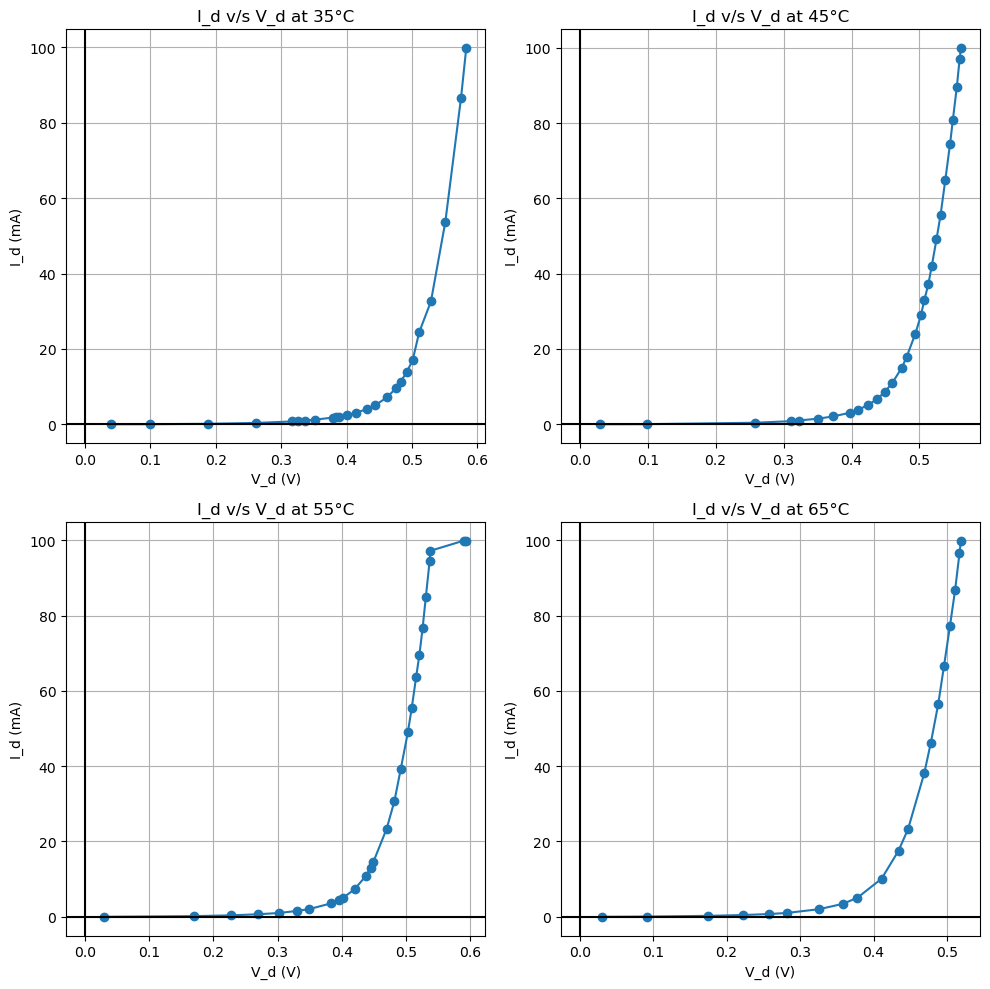
\includegraphics[width=1\linewidth]{Lab_5/Post_Lab/I_d_vs_V_d_Exp_1_Summarised.png}
    \caption{$I_d$ v/s $V_d$ Dark Characteristics for all Temperatures}
\end{figure}

\newpage

\begin{figure}[h!]
    \centering
    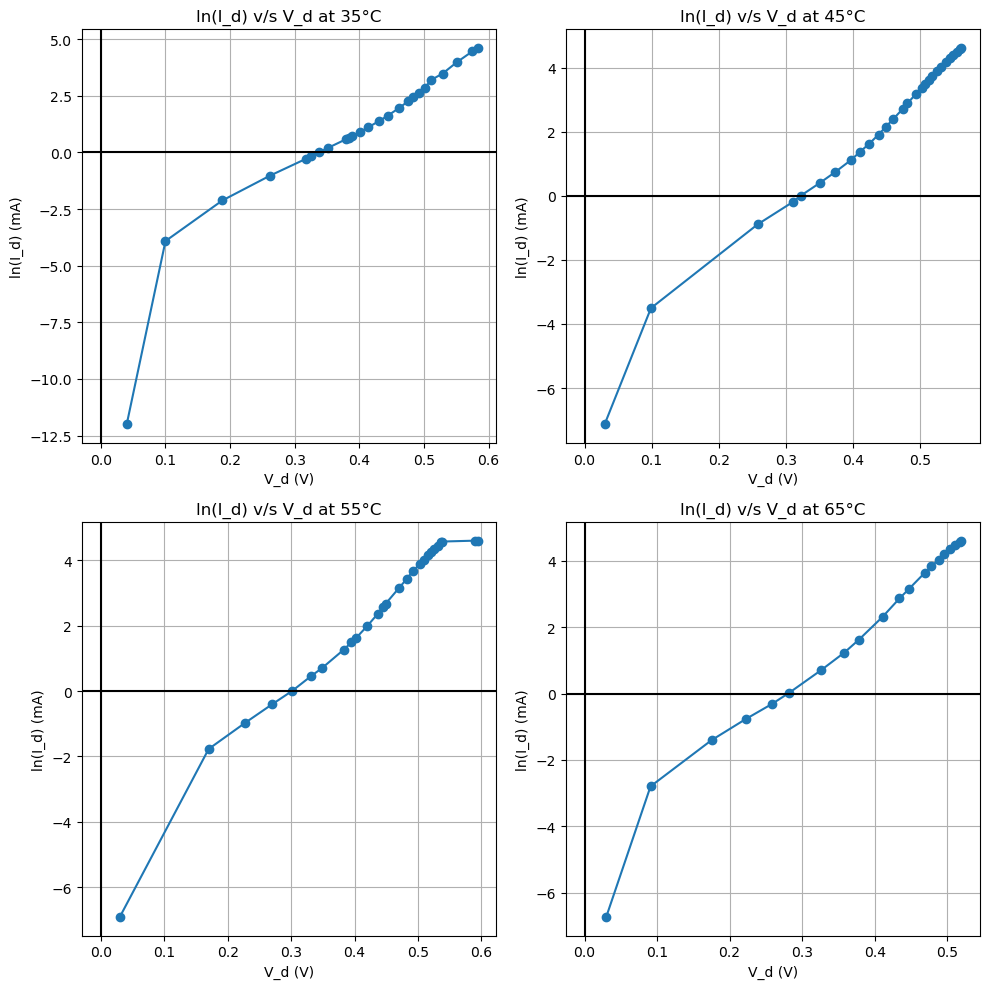
\includegraphics[width=1\linewidth]{Lab_5/Post_Lab/ln_I_d_vs_V_d_Exp_1_Summarised.png}
    \caption{$ln(I_d)$ v/s $V_d$ Dark Characteristics for all Temperatures}
\end{figure}

\subsubsection{Observation Table}
\begin{table}[!h]
    \centering
    \begin{tabular}{|c|c|c|c|c|c|}
        \hline
        \textbf{Temperature} & Vd for Id =1mA & Vd for Id =2mA & Vd for Id =5mA & $\eta$ for low forward bias & $\eta$ for high forward bias \\ \hline
        35 & 0.337 & 0.388 & 0.444 & 1.88 & 1.93 \\ \hline
        45 & 0.322 & 0.373 & 0.424 & 2.33 & 1.99 \\ \hline
        55 & 0.302 & 0.349 & 0.402 & 2.76 & 1.97 \\ \hline
        65 & 0.282 & 0.326 & 0.378 & 2.32 & 2.15 \\ \hline
    \end{tabular}
    \caption{Observations for Experiment 1}
    \label{tab:experiment_1}
\end{table}


\newpage

\subsubsection{Combined Plots}

\begin{figure}[h!]
    \centering
    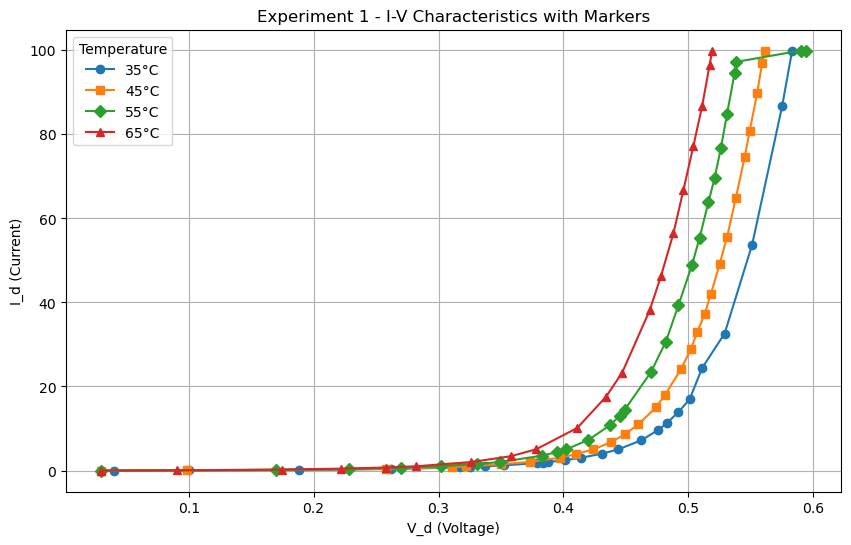
\includegraphics[width=1\linewidth]{Lab_5/Post_Lab/Exp_1_Summarised.png}
    \caption{$I_d$ v/s $V_d$ Dark Characteristics for all Temperatures}
\end{figure}

\begin{figure}[h!]
    \centering
    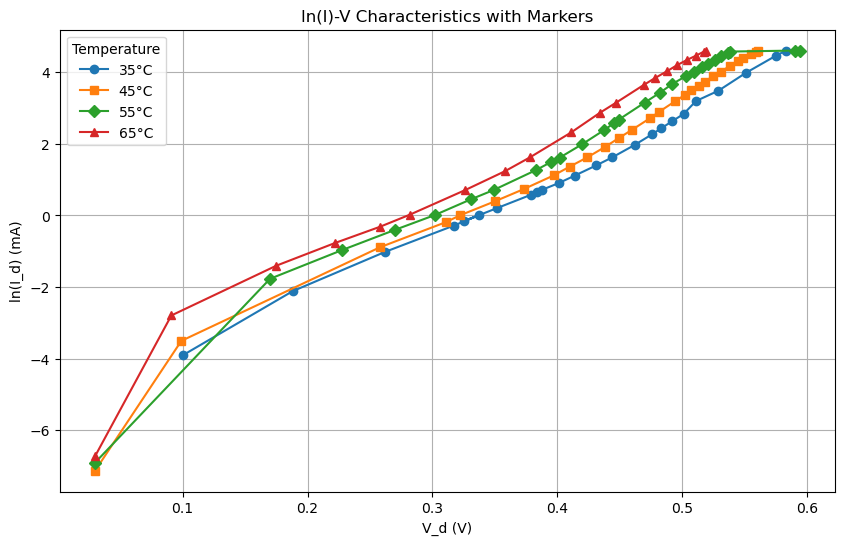
\includegraphics[width=1\linewidth]{Lab_5/Post_Lab/ln_I_d_vs_V_d_Exp_1_Combined.png}
    \caption{Combined plot of $ln(I_d)$ v/s $V_d$ Dark Characteristics for all Temperatures}
\end{figure}



\newpage








%====================================================================================================
%====================================================================================================
%====================================================================================================



\section{Lighted I/V at different temperatures}

\subsection{Aim of the Experiment}
Measure I/V at different temperatures in lighted conditions. Also calculate, Fill Factor at different temperatures.

\subsection{Design}
\begin{figure}[h!]
    \centering
    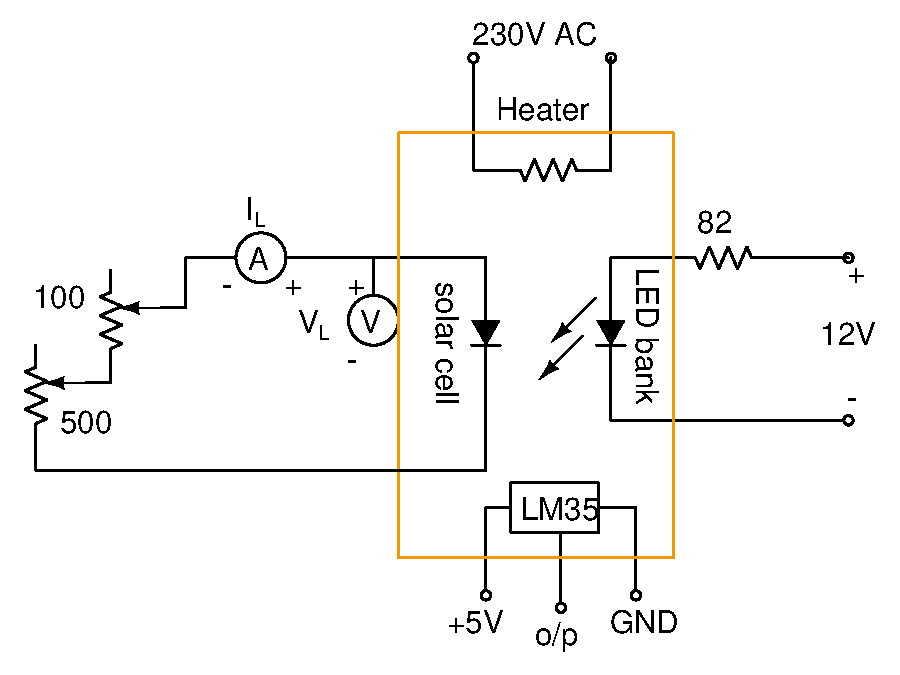
\includegraphics[scale=1]{Ckt_Design_Experiment_2.eps}
    \caption{Caption}
    \label{fig:enter-label}
\end{figure}

\subsection{Simulation}
\subsubsection{Code, Plots, Results}
Included on \hyperlink{page1}{Page 1}, \hyperlink{page2}{Page 2} and \hyperlink{page3}{Page 3} respectively.



\subsection{Experiment}
\newpage
\subsubsection{Individual Plots}
\begin{figure}[h!]
    \centering
    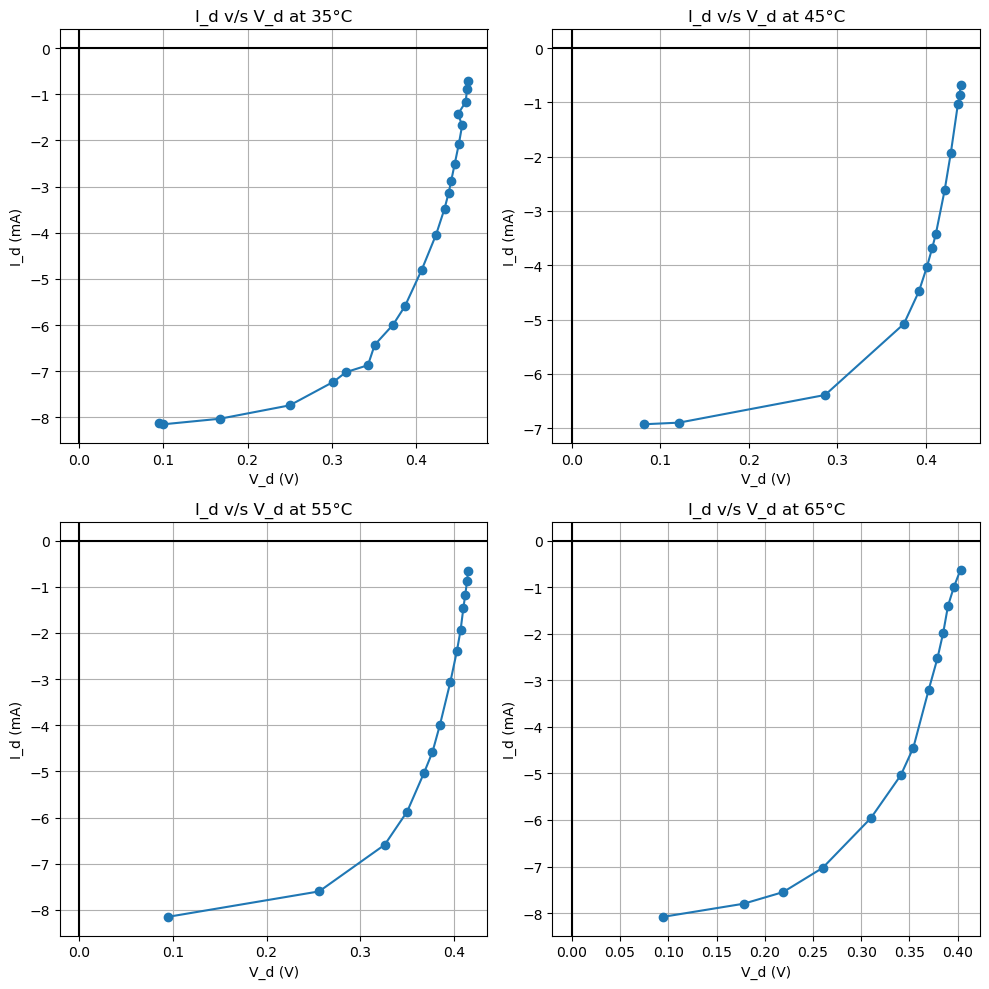
\includegraphics[width=1\linewidth]{Lab_5/Post_Lab/I_d_vs_V_d_Exp_2_Part_1_Summarised.png}
\end{figure}
\begin{figure}[h!]
    \centering
    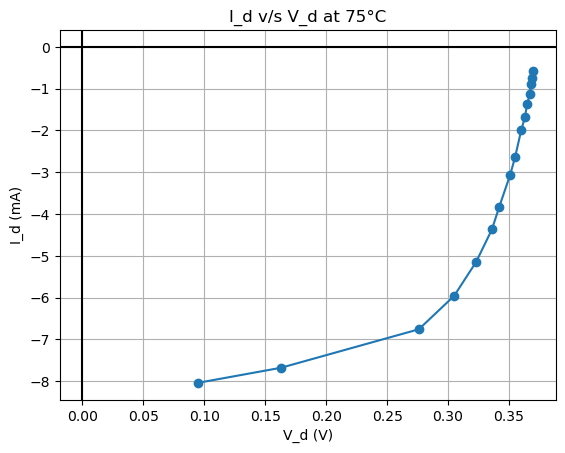
\includegraphics[width=0.6\linewidth]{Lab_5/Post_Lab/I_d_vs_V_d_Exp_2_Part_2_Summarised.png}
\end{figure}
\newpage
\begin{figure}[h!]
    \centering
    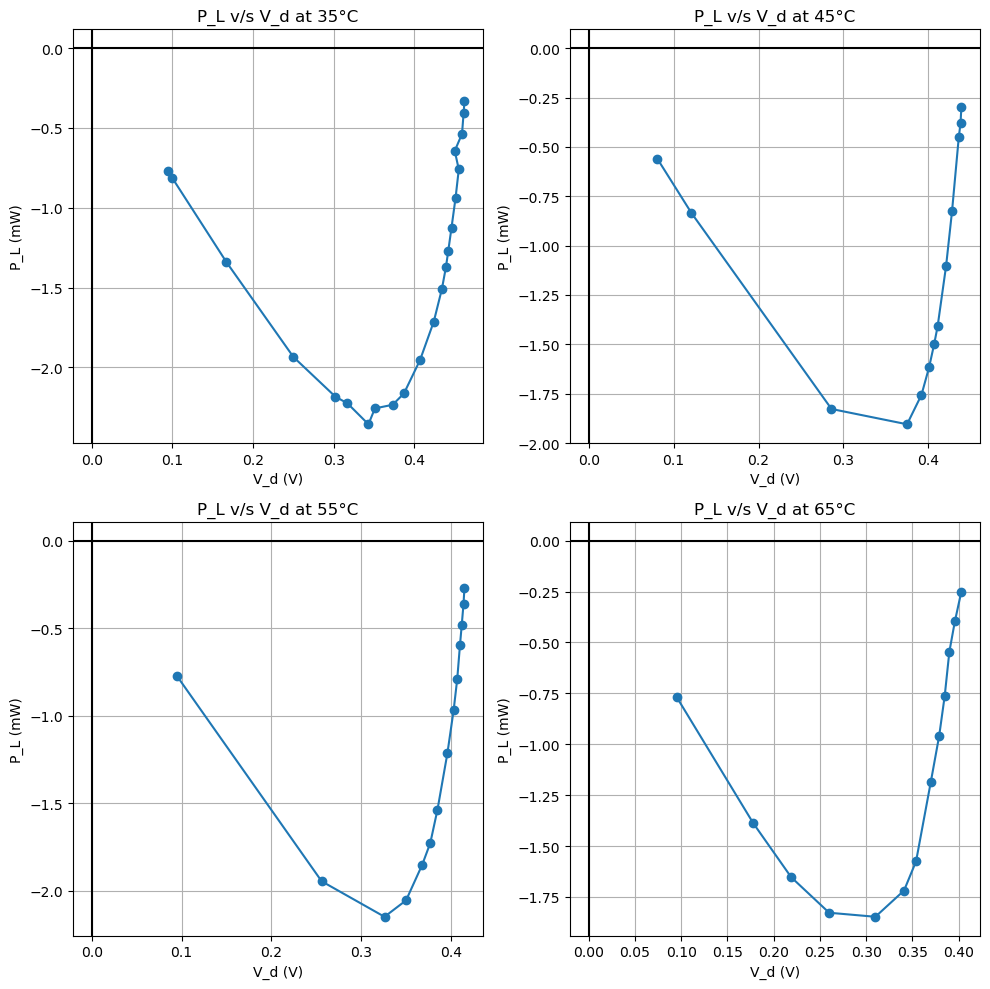
\includegraphics[width=1\linewidth]{Lab_5/Post_Lab/P_L_vs_V_d_Exp_2_Part_1_Summarised.png}
\end{figure}
\begin{figure}[h!]
    \centering
    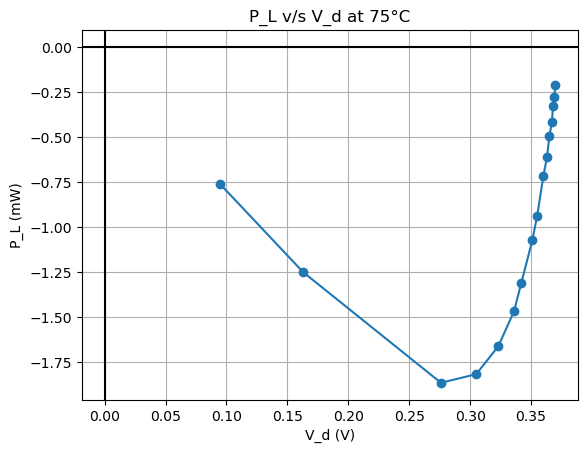
\includegraphics[width=0.6\linewidth]{Lab_5/Post_Lab/P_L_vs_V_d_Exp_2_Part_2_Summarised.png}
\end{figure}

\newpage
\subsubsection{Combined Plots}
\begin{figure}[h!]
    \centering
    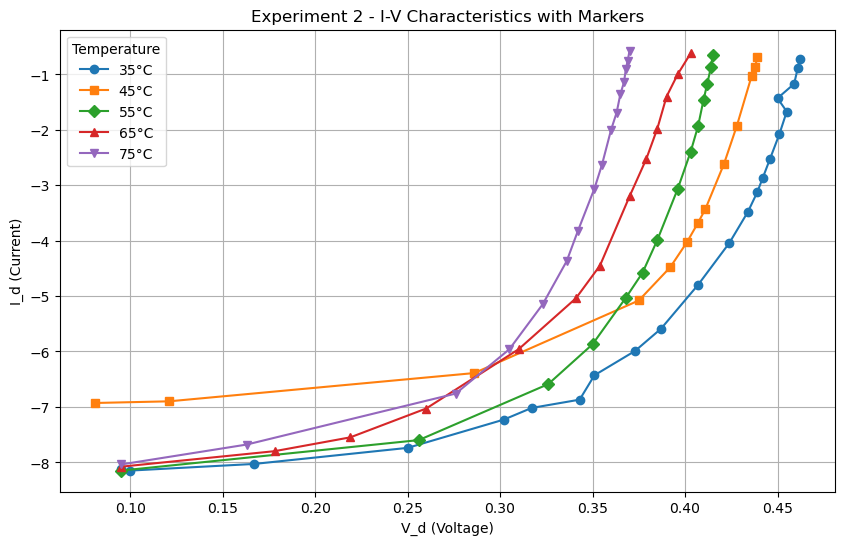
\includegraphics[width=1\linewidth]{Lab_5/Post_Lab/Exp_2_Summarised.png}
    \caption{Combined Plot of $I_L$ v/s $V_L$}
\end{figure}
\begin{figure}[h!]
    \centering
    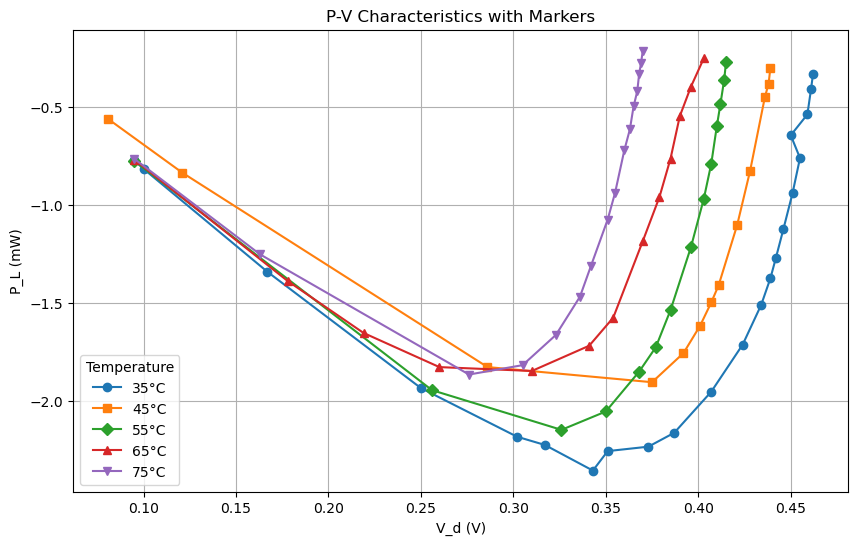
\includegraphics[width=1\linewidth]{Lab_5/Post_Lab/P_L_vs_V_d_Exp_2_Combined.png}
    \caption{Combined Plot of $P_L$ v/s $V_L$}
\end{figure}
\newpage
\begin{figure}[h!]
    \centering
    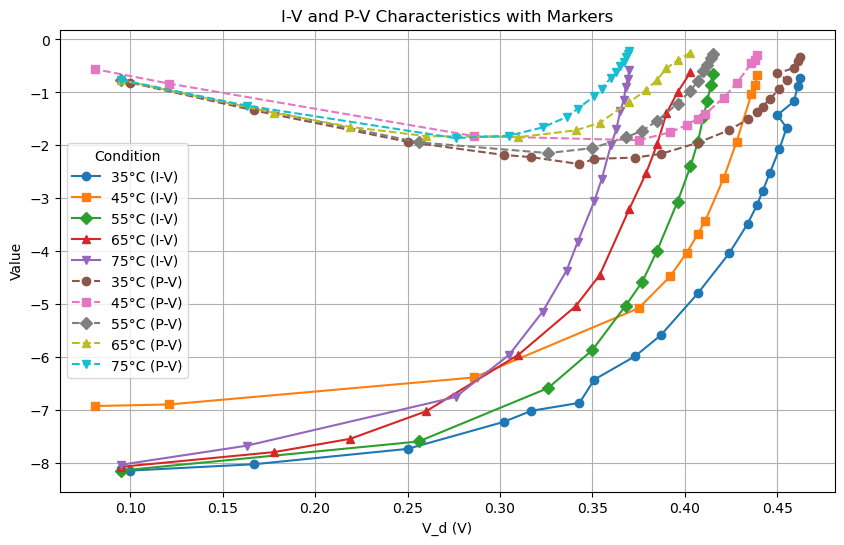
\includegraphics[width=1\linewidth]{Lab_5/Post_Lab/I_L_vs_V_d_and_P_L_vs_V_d_Exp_2_Combined.png}
    \caption{Combined Plot of $I_L$ v/s $V_L$ and $P_L$ v/s $V_L$}
\end{figure}
\begin{figure}[h!]
    \centering
    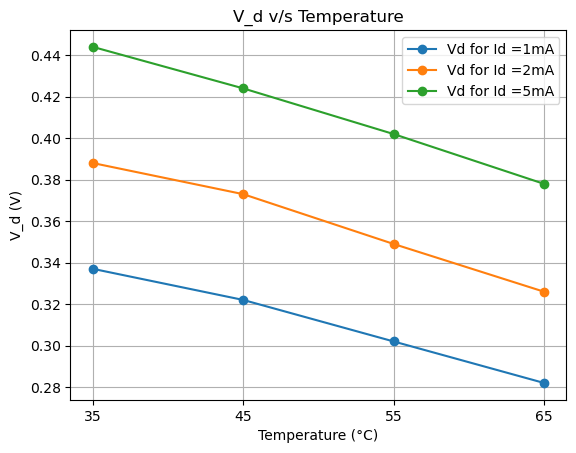
\includegraphics[width=0.7\linewidth]{Lab_5/Post_Lab/V_d_vs_Temperature.png}
    \caption{Combined Plot of $V_d$ v/s Temperature}
\end{figure}
\newpage
\begin{figure}[h!]
    \centering
    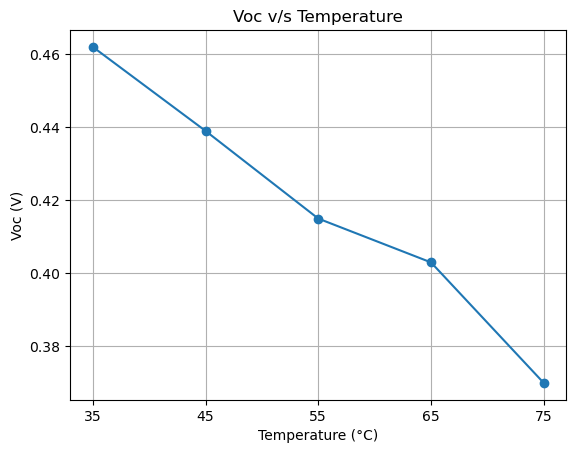
\includegraphics[width=0.7\linewidth]{Lab_5/Post_Lab/V_oc_vs_Temperature.png}
    \caption{Combined Plot of $V_{oc}$ v/s Temperature}
\end{figure}
\begin{figure}[h!]
    \centering
    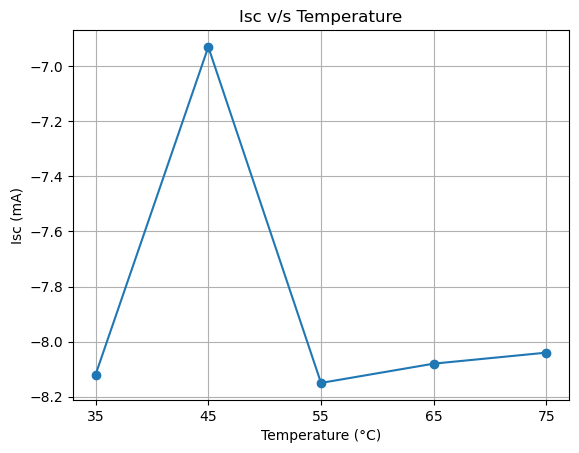
\includegraphics[width=0.7\linewidth]{Lab_5/Post_Lab/V_sc_vs_Temperature.png}
    \caption{Combined Plot of $I_{sc}$ v/s Temperature}
\end{figure}
\newpage
\begin{figure}[h!]
    \centering
    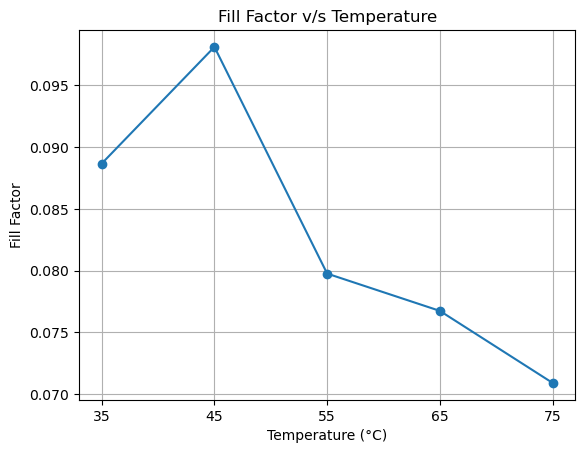
\includegraphics[width=0.7\linewidth]{Lab_5/Post_Lab/Fill_Factor_vs_Temperature.png}
    \caption{Combined Plot of Fill Factor v/s Temperature}
\end{figure}

\subsection{Observations}
It can be clearly concluded from the last 3 graphs, that as the temperature increases, 
\begin{itemize}
    \item $V_d$ decreases
    \item $V_{oc}$ decreases
    \item $I_{sc}$ increases
    \item Fill Factor decreases
\end{itemize}
The jump at 45 $^{\circ}$ Celsius can be attributed to fault in experimental devices or the measuring devices, since we're measuring these things at a very minute scale, where noise can affect our experiments.

\begin{table}[h!]
    \centering
    \begin{tabular}{|c|c|c|c|c|c|c|}
        \hline
        \textbf{Temp (°C)} & \textbf{Isc (mA)} & \textbf{Voc (V)} & \textbf{Im (mA)} & \textbf{Vm (V)} & \textbf{ff} \\ \hline
        35 & -8.12 & 0.462 & -6.87 & 0.343 & 0.6281348 \\ \hline
        45 & -7.93 & 0.439 & -5.80 & 0.375 & 0.6247720 \\ \hline
        55 & -8.15 & 0.415 & -6.59 & 0.326 & 0.6351807 \\ \hline
        65 & -8.08 & 0.403 & -5.96 & 0.310 & 0.5674029 \\ \hline
        75 & -8.04 & 0.370 & -6.76 & 0.276 & 0.6271884 \\ \hline
    \end{tabular}
    \caption{Observation Table for Different Temperatures}
\end{table}
\section{Completion Status}
All the Experiments were completed successfully during lab hours.

\end{document}
